\subsection{Chunks}
As mentioned before one of the most important thinks for the terrain was a way to edit it.
Editing the whole terrain at once would be very slow and not very efficient.
Thus the terrain is split into chunks - cubes with side length 16.
Each chunk is a separate object and can be edited independently.
This solution is much more efficient but is also causes some problems.

One problem is that the terrain is not continuous.
Every time we edit a chunk we need to make sure that the edges of the chunk are the same as the edges of the neighboring chunks.
This is done by making sure that when a function that updates one chunk is called it is also called with the exact same parameters for other affected chunks.
Without this the terrain would have holes in it between chunks which is shown in a screenshot from an early version of the game in \autoref{fig:gaps_between_chunks}.

Another problem is that the algorithm we used for generating the terrain, described in \autoref*{subsec:marching_cubes}, calculates normal vectors based on the values of the scalar field around the point at which the normal is calculated.
This means that that the normal vectors at the edges of the chunks have to be calculated differently.
This is a common problem with the algorithm and it is visualized in \autoref*{fig:problem_with_normals_at_chunk_edge}.
The most common solution and the one we used is extending the scalar field by one layer of points around the chunk.
This means that the chunk contains the information about the scalar field outside of the chunk itself.
That way the normal vectors can be calculated the same way for all points in the chunk.

\begin{figure}[H]
    \centering
    \begin{minipage}{0.45\textwidth}
        \centering
        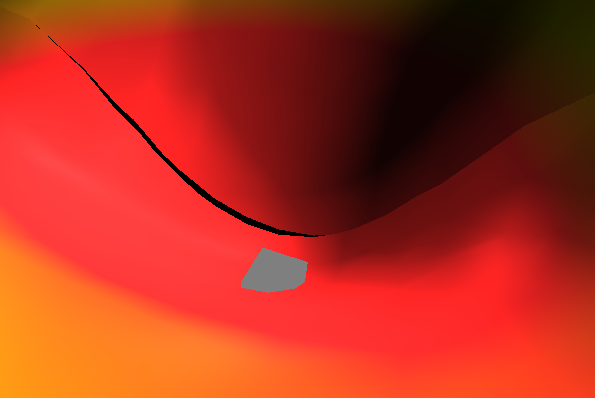
\includegraphics[width=0.8\textwidth]{chapters/system_architecture/sections/terrain_generation/resources/chunk_edges_gaps.png}
        \caption{Gaps between chunks.}
        \label{fig:gaps_between_chunks}
    \end{minipage}\hfill
    \begin{minipage}{0.45\textwidth}
        \centering
        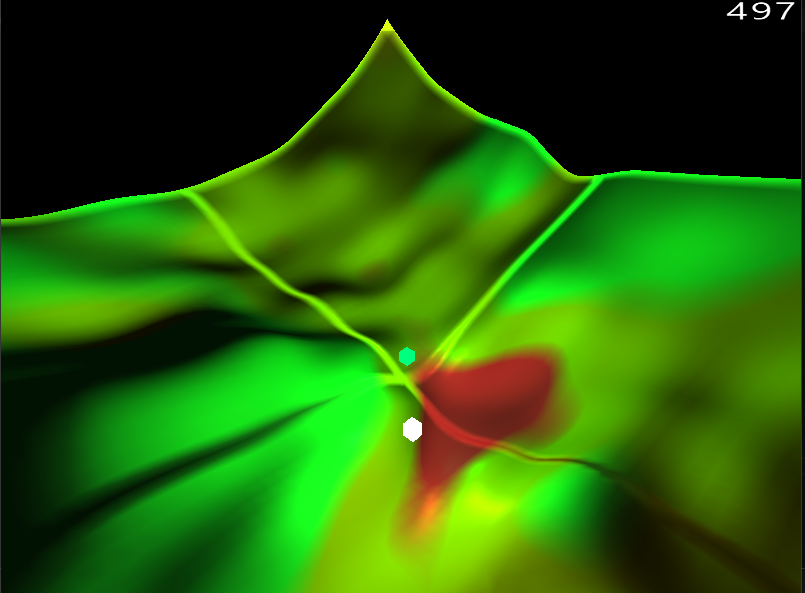
\includegraphics[width=0.8\textwidth]{chapters/system_architecture/sections/terrain_generation/resources/chunk_edges_normals_problem.png}
        \caption{Problem with normals at chunk edges.}
        \label{fig:problem_with_normals_at_chunk_edge}
    \end{minipage}
\end{figure}